\documentclass{article}

\usepackage[a4paper]{geometry}
\usepackage{listings}
\usepackage{xcolor}
\usepackage[utf8]{inputenc}
\usepackage{pdflscape}
\usepackage{multicol}
\usepackage{pdfpages}
\usepackage{pdflscape}

\usepackage{hyperref}
\hypersetup{
%	colorlinks=false, %set true if you want colored links
	linktoc=all,     %set to all if you want both sections and subsections linked
%	linkcolor=blue,  %choose some color if you want links to stand out
}

\newcommand{\teamname}{Oachkatzlschwoaf}
\newcommand{\teammembers}{Markus Hasenöhrl, Thomas Tangl, Gregor Matl}
\newcommand{\competition}{NWERC 2016}

\pdfinfo{
	/Title (Cheatsheet Team \teamname) % sofern wir den namen nehmen
	/Creator (TeX)
	/Author (\teammembers)
	/Subject (Cheatsheet for \competition)
}

% This sets page margins to .5 inch if using letter paper, and to 1cm
% if using A4 paper. (This probably isn't strictly necessary.)
% If using another size paper, use default 1cm margins.
\geometry{top=22mm,left=8mm,right=8mm,bottom=10mm}

% Turn off header and footer
\pagestyle{empty}

% Redefine section commands to use less space
\makeatletter
\renewcommand{\section}{\@startsection{section}{1}{0mm}%
	{-1ex plus -.5ex minus -.2ex}%
	{0.5ex plus .2ex}%x
	{\normalfont\large\bfseries}}
\renewcommand{\subsection}{\@startsection{subsection}{2}{0mm}%
	{-1explus -.5ex minus -.2ex}%
	{0.5ex plus .2ex}%
	{\normalfont\normalsize\bfseries}}
\renewcommand{\subsubsection}{\@startsection{subsubsection}{3}{0mm}%
	{-1ex plus -.5ex minus -.2ex}%
	{1ex plus .2ex}%
	{\normalfont\small\bfseries}}
\makeatother

% Don't print section numbers
\setcounter{secnumdepth}{0}


%\setlength{\parindent}{0pt}
%\setlength{\parskip}{0pt plus 0.5ex}

\usepackage{fancyhdr}
\pagestyle{fancy}
\setlength{\headheight}{0pt} 
\lhead{\textsc{Technische Universit\"at M\"unchen}\vskip-8mm}
\renewcommand{\headrulewidth}{0pt}
\rhead{\textsc{\thepage}\vskip-8mm}
\fancyfoot[C]{\vskip-8mm\textsc{\thepage}}

\begin{document}
\begin{landscape}
\raggedright
\footnotesize
\begin{multicols}{2}
	
	
	% multicol parameters
	% These lengths are set only within the two main columns
	%\setlength{\columnseprule}{0.25pt}
	\setlength{\premulticols}{1pt}
	\setlength{\postmulticols}{1pt}
	\setlength{\multicolsep}{1pt}
	\setlength{\columnsep}{10pt}
	
	\begin{center}
		\Large{
			Team Reference Document\\
			\underline{Team \texttt{\teamname}, TU M\"unchen}\vskip0.05cm 
			North West European Programming Contest 2016} \vskip0.9cm
	\end{center}
	
	\begin{multicols}{3}
		\tableofcontents
	\end{multicols}
	
%	\vfill 

\lstset{
  belowcaptionskip=1\baselineskip,
  breaklines=true,
  frame=single,
%  xleftmargin=\parindent,
  language=C++,
  showstringspaces=false,
  basicstyle=\footnotesize\ttfamily,
  keywordstyle=\bfseries\color{blue},
  commentstyle=\color{green!50!black},
  identifierstyle=\bfseries\color{black},
  stringstyle=\color{orange},
  numbers=none,
  numbersep=5pt,
  numberstyle=\tiny\color{gray!15!black},
  %title=\lstname
}
\section{Graph Algorithms}

\subsection{SCC}
\lstinputlisting{source_codes/SCC.cpp}

\subsection{EulerianPath}
\lstinputlisting{source_codes/EulerianPath.cpp}

\subsection{ArticulationPoints}
\lstinputlisting{source_codes/ArticulationPoints.cpp}

\subsection{MinCostMaxFlow}
\lstinputlisting{source_codes/MinCostMaxFlow.cpp}

\subsection{MaxFlow: PushRelabel}
\lstinputlisting{source_codes/PushRelabel.cpp}

\subsection{MaxFlow: Dinic}
\lstinputlisting{source_codes/MaxflowDinic.cpp}

\subsection{MinCostMatching}
\lstinputlisting{source_codes/MinCostMatching.cpp}

\subsection{MaxBipartiteMatching}
\lstinputlisting{source_codes/MaxBipartiteMatching.cpp}

\subsection{MinCut}
\lstinputlisting{source_codes/MinCut.cpp}


\section{Trees}

\subsection{Segment Tree}
\lstinputlisting{source_codes/SegmentTree.cpp}
\subsection{BIT}
\lstinputlisting{source_codes/BIT.cpp}

\subsection{BIT2D}
\lstinputlisting{source_codes/BIT2D.cpp}

\subsection{RMQDP}
\lstinputlisting{source_codes/RMQDP.cpp}

\subsection{OrderStatisticsTree}
\lstinputlisting{source_codes/OrderStatisticsTree.cpp}

\subsection{LCA}
\lstinputlisting{source_codes/LCA.cpp}

\subsection{DP in Tree}
\lstinputlisting{source_codes/DPTREE.cpp}

\section{Geometry}

\subsection{ConvexHull}
\lstinputlisting{source_codes/ConvexHull.cpp}

\subsection{Geometry}
\lstinputlisting{source_codes/Geometry.cpp}

\subsection{Delaunay Triangulation}
\lstinputlisting{source_codes/DelauneyTriangulation.cpp}

\section{Math}

\subsection{NumberTheory}
\lstinputlisting{source_codes/NumberTheory.cpp}

\subsection{RabinMiller}
\lstinputlisting{source_codes/RabinMiller.cpp}

\subsection{GaussJordan}
\lstinputlisting{source_codes/GaussJordan.cpp}

\subsection{FFT}
\lstinputlisting{source_codes/FFT.cpp}

\section{Strings}

\subsection{SuffixArray}
\lstinputlisting{source_codes/SuffixArray.cpp}

\subsection{Z-Algorithm}
\lstinputlisting{source_codes/ZAlgorithm.cpp}

\subsection{KMP}
\lstinputlisting{source_codes/KMP.cpp}

\subsection{IO}
\lstinputlisting{source_codes/IO.cpp}

\section{Miscellaneous}

\subsection{Divide and Conquer Optimization}
\lstinputlisting{source_codes/DivConquer.cpp}

\subsection{C++ IO (Gregor)}
\lstinputlisting{source_codes/GregorCPPIO.cpp}

\subsection{GCC Builtin Functions}
\lstinputlisting{source_codes/GCCBuiltinFunctions.cpp}

\subsection{Longest Increasing Subsequence}
\lstinputlisting{source_codes/LongestIncreasingSubsequence.cpp}

\subsection{Longest Palindrome}
\lstinputlisting{source_codes/LongestPalindrome.cpp}

\section{Theorems}
\paragraph{Euler’s theorem.} For any planar graph, $V - E + F = 1 + C$, where $V$ is the number of graph's vertices, $E$ is the number of edges, $F$ is the number of faces in graph's planar drawing, and $C$ is the number of connected components. Corollary: $V-E+F=2$ for a 3D polyhedron.

\paragraph{Vertex covers and independent sets.} Let $M, C, I$ be a max matching, a min vertex cover, and a max independent set. Then $|M| \le |C| = N -|I|$, with equality for bipartite graphs. Complement of an MVC is always a MIS, and vice versa. Given a bipartite graph with partitions $(A,B)$, build a network: connect source to $A$, and $B$ to sink with edges of capacities, equal to the corresponding nodes' weights, or 1 in the unweighted case. Set capacities of the original graph's edges to the infinity.
Let $(S, T)$ be a minimum $s-t$ cut. Then a maximum(-weighted) independent set is $I = (A \cap S)\cup(B \cap T)$,
and a minimum(-weighted) vertex cover is $C = (A - T) \cup (B \cap S)$.

\paragraph{2-SAT.} Build an implication graph with 2 vertices for each variable - for the variable and its inverse; for each clause $x \lor y$ add edges $(\neg x, y)$ and $(\neg y, x)$. The formula is satisfiable if $x$ and $\neg x$ are in distinct SCCs, for all $x$. To find a satisfiable assignment, consider the graph's SCCs in topological order from
sinks to sources (i.e. Kosaraju's last step), assigning `true' to all variables of the current SCC (if it hasn't been previously assigned `false'), and `false' to all inverses.

\paragraph{Pick’s theorem.} $I = A - B/2 + 1$, where $A$ is the area of a lattice polygon, $I$ is number of lattice points inside it, and $B$ is number of lattice points on the boundary. Number of lattice points minus one on a line segment from $(0, 0)$ and $(x, y)$ is $gcd(x, y)$.

\subsection{Combinatorics}
\paragraph{Mathematical Sums}
\bgroup
\def\arraystretch{1.2}
\begin{tabular}{l l}
	$\sum_{k=0}^n k=n(n+1)/2$&	$\sum_{k=a}^b k=(a+b)(b-a+1)/2$\\
	$\sum_{k=0}^n k^2=n(n+1)(2n+1)/6$&	$\sum_{k=0}^n k^3=n^2(n+1)^2/4$\\
	$\sum_{k=0}^n k^4=(6n^5+15n^4+10n^3-n)/30$&	$\sum_{k=0}^n k^5=(2n^6+6n^5+5n^4-n^2)/12$\\
	$\sum_{k=0}^n x^k=(x^{n+1}-1)/(x-1)$&	$\sum_{k=0}^n kx^k=(x-(n+1)x^{n+1}+nx^{n+2})/(x-1)^2$\\
\end{tabular}
\egroup
%\paragraph{Mathematical Sums}

\paragraph{Burnsides Lemma.} The number of orbits under Group $G$'s action on set $X$:\\
$|X/G|=\frac{1}{|G|}\sum_{g\in G}|X_g|$, where $X_g = \{x \in X : g(x) = x\}$ ("Average number of fixed points.")\\
Let $w(x)$ be weight of $x$'s orbit. Sum of all orbit's weights: $\sum_{o \in X/G}w(o)=\frac{1}{|G|}\sum_{g\in G}\sum_{x\in X_g}w(x)$.

\paragraph{Simpson Formula.}
$\int_{a}^{b}f(x)dx = \frac{b-a}{6}(f(a)+4f(\frac{a+b}{2})+f(b))$.\\
Error: $|E(f)| \leq \frac{(b-a)^5}{2880} \max\limits_{a\leq x\leq b}|f^{(4)}(x)|$.

\section[More Theorems]{}
\end{multicols}
\end{landscape}

\includepdf[scale=0.95, angle=270, landscape=true,pages={2},clip,trim=0mm 0mm 0mm 6cm,offset=0mm -1cm,pagecommand={\thispagestyle{fancy}}]{notebook_cat_us_trophy}

\includepdf[scale=0.95, angle=270, landscape=true,pages={3},clip,trim=0mm 0mm 0mm 20mm,offset=0mm -10mm,pagecommand={\thispagestyle{fancy}}]{notebook_cat_us_trophy}

\includepdf[scale=0.95, angle=270, landscape=true,pages={7},clip,trim=0mm 0mm 0mm 7cm,offset=0mm -1cm,pagecommand={\thispagestyle{fancy}}]{notebook_cat_us_trophy}

\includepdf[scale=0.95, angle=270, landscape=true,pages={8},clip,trim=0mm 1.2cm 0mm 20mm,offset=0mm -10mm,pagecommand={\thispagestyle{fancy}}]{notebook_cat_us_trophy}

\includepdf[scale=0.95, angle=270, landscape=true,pages={18},clip,trim=0mm 0mm 0mm 8cm,offset=0mm -1cm,pagecommand={\thispagestyle{fancy}}]{notebook_cat_us_trophy}

\end{document}
